% thesis.tex
%
% This file is root file for an example thesis written using the
% IIT Bombay LaTeX Style file.
% Created by Amey Karkare (21 June 2007)
%
% It is provided without warranty on an AS IS basis.

%=====================================================================
% Read: http://www.cse.iitb.ac.in/karkare/iitbthesis/
%    FAQ.txt     for frequently asked quetions
%    Changes.txt for changes
%    README      for more information
%=====================================================================

%=====================================================================
% DOCUMENT STYLE
%=====================================================================
% IITB PhD Thesis format default settings are:
%   12pt, one-sided printing on a4 size paper
\documentclass{RAITreport}
% For two-sided printing, with Chapter starting on odd-numbered pages,
% use the following line instead:
%%\documentclass[openright,twoside]{iitbthesis}

%=====================================================================
% OPTIONAL PACKAGES
%=====================================================================
% To include optional packages, use the \usepackage command.
% For e.g., The package epsfig is used to bring in the Encapsulated
%    PostScript figures into the document.
%    The package times is used to change the fonts to Times Roman;
%=====================================================================
\usepackage{epsfig}
\usepackage{times}
%\usepackage{psfig}
%=====================================================================
%  Single counter for theorems and theorem-like environments:
%=====================================================================
\newtheorem{theorem}{Theorem}[chapter]
\newtheorem{assertion}[theorem]{Assertion}
\newtheorem{claim}[theorem]{Claim}
\newtheorem{conjecture}[theorem]{Conjecture}
\newtheorem{corollary}[theorem]{Corollary}
\newtheorem{definition}[theorem]{Definition}
\newtheorem{example}[theorem]{Example}
\newtheorem{figger}[theorem]{Figure}
\newtheorem{lemma}[theorem]{Lemma}
\newtheorem{prop}[theorem]{Proposition}
\newtheorem{remark}[theorem]{Remark}

%=====================================================================
% End of Preamble, start of document
%

\begin{document}

%=====================================================================
% Include the prelude for Title page, abstract, table of contents, etc
% You need to modify it to contain your details
% prelude.tex
%   - titlepage
%   - dedication (optional)
%   - approval sheet
%   - course certificate
%   - table of contents, list of tables and list of figures
%   - nomenclature
%   - abstract
%============================================================================


\clearpage\pagenumbering{roman}  % This makes the page numbers Roman (i, ii, etc)



% TITLE PAGE
%   - define \title{} \author{} \date{}
\title{Wolff Parkinson White Syndrome Detection}
\author{Shabbir Talib 20CE1095\\Atharva Hirve 20CE1086\\Jay Dandekar 20CE1103\\Deyush Kulkarni 20CE1008}
\date{April 2023}

%  - Roll number, required for title page, approval sheet, and
%    certificate of course work
%\rollnum{02405003}

%   - The default degree is ``Doctor of Philosophy''
%     (unless the document style msthesis is specified
%      and then the default degree is ``Master of Science'')
%     Degree can be changed using the command \iitbdegree{}
%\iitbdegree{Master \TeX nician}

%   - The default report type is preliminary report.
%      * for a PhD thesis, specify \thesis
%\thesis
%      * for a M.Tech./M.Phil./M.Des./M.S. dissertation, specify \dissertation
%\dissertation
%      * for a DIIT/B.Tech./M.Sc.project report, specify \project
%\project
%      * for any other type, use  \reporttype{}
%\reporttype{ReportType}

%   - The default department is ``Unknown Department''
%     The department can be changed using the command \department{}
\department{Department of Computer Engineering}

%    - Set the guide's name
\setguide{Mrs. Tabassum Maktum}
\setprojectcoordinatorname{Dr. Aditi Chhabria}
%    - Set the coguide's name (if you have one)
%\setcoguide{Prof Amitabha Sanyal}
%    - Set external guide (if you have one)
%\setexguide{Prof External Guide}

%   - once the above are defined, use \maketitle to generate the titlepage
\maketitle

%--------------------------------------------------------------------%
% DEDICATION
%   Dedications, if any, must be first page after title page.
%\begin{dedication}
%To my family
%\end{dedication}

%--------------------------------------------------------------------%
% APPROVAL SHEET
%   - for final thesis, you need Approval Sheet. So, uncomment the
%     \makeapproval command.
%     it should come after dedication, if dedication is
%     present. Otherwise it is the first page after title page.
\certificate

\makeapproval

%--------------------------------------------------------------------%
% DECLARATION PAGE
%   - To include a declaration page

%--------------------------------------------------------------------%


\begin{declaration}
\begin{center}
\Large \bf {DECLARATION}
\end{center}

%\begin{flushleft}
\noindent
We declare that this written submission represents our ideas and does not involve plagiarism.  We have
adequately cited and referenced the original sources wherever others' ideas or words have been included. We also declare
that we have adhered to all principles of academic honesty and
integrity and have not misrepresented or fabricated or falsified any
idea/data/fact/source in our submission. We understand that any
violation of the above will be cause for disciplinary action against us by the
Institute and can also evoke penal action from the sources which
have thus not been properly cited or from whom proper permission has
not been taken when needed.
%\end{flushleft}

\end{declaration}







%--------------------------------------------------------------------%
% COPYRIGHT PAGE
%   - To include a copyright page use \copyrightpage
% \copyrightpage

%--------------------------------------------------------------------%
% ABSTRACT
\begin{abstract}
  %\input{abstract}
%  Here is my introduction text. The section heading is in a large bold
%font and all sections and subsections are numbered.
%
%Type your main text in 12-point Times with 1.5 line spacing. Do not
%use double-spacing. All paragraphs should be indented 1 pica
%(approximately 1/6- or 0.17-inch or 0.422 cm). Be sure your text is
%fully justified---that is, flush left and flush right. Please do not
%place any additional blank lines between paragraphs.

In the present day and age, we live in a world where anything and everything related to medical condition/syndrome detection and treatment has and continues to become extremely crucial. The dependency on all such systems has grown rapidly in the last few decades due to number of external factors, of the critical factor being these system’s capability and capacity of detecting diseases and syndromes or any other prevalent conditions well-in time. This offers patients the chance of exploring further options. These options depend on severity of detection if any, further course of treatment and other factors associated with the same. The team has developed a web application for analyzing ECGs of patients and detection of Wolff Parkinson White syndrome through irregular heartbeat and other pre-set parameters, in the process providing additional and useful information including symptoms, precautions and possible mode of treatments. Also, providing patients with connections to concerned health centers in the process of creating a one-stop solution for this syndrome. 
\end{abstract}


%--------------------------------------------------------------------%
% CONTENTS, TABLES, FIGURES
\tableofcontents
\listoftables
\listoffigures


%--------------------------------------------------------------------%


\cleardoublepage\pagenumbering{arabic} % Make the page numbers Arabic (1, 2, etc)


%=====================================================================
% Include the technical part of the report
 \chapter{Introduction}
\section{Overview}\label{sec1}
%\subsection{AI \& ML}\label{subsec1}

%\subsubsection{Data Science}

WPW syndrome (Wolff-Parkinson-White syndrome) is a cardiac arrhythmia characterized by an abnormal pathway between the atria and ventricles of the heart, which can lead to a rapid and irregular heartbeat. The condition is usually diagnosed using an electrocardiogram (ECG), which measures the electrical activity of the heart. However, WPW syndrome is often associated with low detection rates which increases the criticality of this syndrome and emphasizing the importance of early detection. The low detection rate of WPW syndrome can be attributed to several factors. One of the primary reasons is that the condition is often asymptomatic, meaning that many people with WPW syndrome may not experience any noticeable symptoms. In some cases, WPW syndrome may only be discovered incidentally during routine medical tests such as an electrocardiogram (ECG).  

Another reason for the low detection rate of WPW syndrome is that it is a relatively rare condition. According to some estimates, WPW syndrome affects only around 0.1-0.3\% of the general population. As a result, many healthcare providers may not be familiar with the condition or may not consider it as a possible diagnosis in patients with symptoms that can be attributed to other causes. In addition to the listed parameters, WPW syndrome can be difficult to diagnose, especially in cases where the extra pathway is intermittent or only present during certain heart rhythms. In some cases, additional testing such as a Holter monitor or electrophysiological study may be necessary to detect the condition. 



Overall, the low detection rate of WPW syndrome underscores the importance of regular medical check-ups and screenings, especially for individuals with a family history of the condition or other risk factors. If a patient is experiencing symptoms such as rapid or irregular heartbeats, it is important to seek medical attention promptly to rule out any underlying cardiac conditions.  




\newpage

This gives an overview \cite{kunjir2017data} about chapter. The following Equation~\ref{eq2} about parameters.

 The following Figure~\ref{fig:rait-dypu-logo} is the DYPU Logo.

\begin{figure}[h]
	\centering
		
\includegraphics{rait-dypu-logo.png}
	\caption{DY Patil Deemed University logo}
	\label{fig:rait-dypu-logo}
\end{figure}


%\begin{figure}[h]
%	\centering
%	
\includegraphics[width=0.7\linewidth]{rait-dypu-logo}
%	\caption{Figure Caption Here}
%	\label{fig:plot}
%\end{figure}


\begin{equation} \label{eq1}
	\beta \leftarrow \frac{5 (\pi - 1)}{\lambda^2} 
\end{equation}




\cite{kunjir2017data}



\begin{enumerate}
	\item Which observations strongly motivated you to take up this problem domain to work.
	
	\item Which observations strongly motivated you to take up this problem domain to work.
\end{enumerate}

\begin{description}
	\item[AI] Which observations strongly motivated you to take up this problem domain to work.
\end{description}

\begin{center}	
	Which observations strongly motivated you to take up this problem domain to work.
\end{center}


The following Table~\ref{tab1} shows the Name of the Students.
\begin{table}[!ht] \label{tab1}
	\caption{Name of Students}
	\centering
	\begin{tabular}{|p{5cm}|p{5cm}|}
		\hline
		\textbf{Name}                  & \textbf{Roll No.} \\ \hline
		Mr. Kishor Deepak Waghe        & (20CE5009)        \\ \hline
		Mr. Pradyumna Sameer Mandawkar & (20CE5010)        \\ \hline
		Ms. Prabhuti Jayesh Patil      & (20CE5014)        \\ \hline
		Which observations strongly motivated you to take up this problem domain to work.      & (19CE1053)        \\ \hline
	\end{tabular}
\end{table}

\section{Motivation}
There has been a visible and drastic change towards a positive side when it comes to how the healthcare sector has adapted to the evolution of technology. The COVID-19 pandemic further accelerated the need for use of remote systems when dealing with patient of any kind. This is where the proposed system comes into the picture ensuring an easily available, cost and time sensitive solution for patients who may be suffering from the Wolff Parkinson White Syndrome. The motivation behind selection and development of this system is: 


\begin{itemize}
	\item Firstly, it could help in the early and accurate diagnosis of this very rare condition, which is important for effective treatment. 
	\item Secondly, it could improve the speed and efficiency of diagnosis, particularly in settings where access to medical professionals or resources is limited. 
	\item A machine learning model could potentially use a large dataset of ECG recordings to identify patterns or features that are associated with WPW syndrome. 
	\item The model could also be designed to provide a probability score or confidence level for its classification, allowing medical professionals to make more informed decisions about treatment. 
	\item However, it's important to note that developing a machine learning model for diagnosing WPW syndrome would require a large, diverse and representative dataset of ECG recordings, as well as appropriate regulatory approvals and ethical considerations.  
	\item Additionally, the machine learning model should be used in conjunction with trained medical professionals, as it is intended to assist with diagnosis and improve patient outcomes. 
\end{itemize}


\section{Problem Statement and Objectives}
The primary objectives of our web-application would be to provide:  
\begin{enumerate}
	\item Provides streamlined way for individuals to perform a quick check up. 
	\item The first part of our project is to create a separate model that will be used to convey if the patient needs to take an ECG test in the first place.
	\item The mentioned model is based on symptoms that a person with a heart problem and in need of check-up might suffer from. 
	\item The various symptoms are as follows: 
	\begin{itemize}
		\item High heart rate 
		\item Dizziness 
		\item Fainting 
		\item Constant Tiredness (Fatigue) 
		\item Anxiousness			 
		\item Chest Pain 
		\item Difficulty Breathing
	\end{itemize}
	\item The inputs the user will provide will be yes/no if they suffer from the above-mentioned symptoms. 
	\item Using the above inputs, the project will provide a prompt if they should undergo an ECG test. 
	\item The core element of our project is to develop a model such that by taking the ECG data input, can detect if the person is suffering from Wolff-Parkinson-White Syndrome. 
	\item The next part of the project is to provide a list of medical centers where the user can go for treatment if needed. 
	\item And another part would be to display the various available treatments they can take if they suffer from Wolff-Parkinson-White Syndrome.
	 
	
\end{enumerate}

\section{Organization of the report}

The report is organised as follows: The Chapter 2 reviews the literature. Chapter 3 focuses on defining the system's issue. That includes problem categorization, proposed technologies, device architecture, and hardware/software requirements. On the other hand, Chapter 5 describes the inference and future work on the technique to be utilized as a more improved model.
\add{text}
 \include{Chap2}
 \include{Chap3}
 \include{Chap4}
 \include{Chap5}
 \addcontentsline{toc}{chapter}{References}
 \renewcommand{\bibname}{References}\thispagestyle{plain}
 
 

              
%=====================================================================
% APPENDIX
%  Appendices, if any, must precede the cited literatures.
%  Appendices shall be numbered in Roman Capitals (e.g. Appendix IV)
%
%% \appendix
%% \include{appendix_something}

%=====================================================================
% BIBLIOGRAPHY
%   This should follow the appendices, if any, otherwise summary and
%   conclusions chapter.
% Choose your bibliography style
% plain is the basic style, others include ieeetr, siam, asm, etc
\bibliographystyle{IEEEtr}
% Add the bib file
\bibliography{san}
\newpage
\begin{center}
	\vspace*{11cm}
	\centering
	{  \huge \bfseries Appendices}
\end{center}

\let\cleardoublepage\clearpage
\appendix
\chapter{Weekly Progress Report}
\begin{figure}[h]
	\centering
	
\includegraphics[width=10cm, height=5cm]{rait-dypu-logo.png}
	\caption[Weekly Progress Report]{Weekly Progress Report}
	\label{fig:my_label}
\end{figure}
\newpage
\chapter{Plagiarism Report}\thispagestyle{plain}
%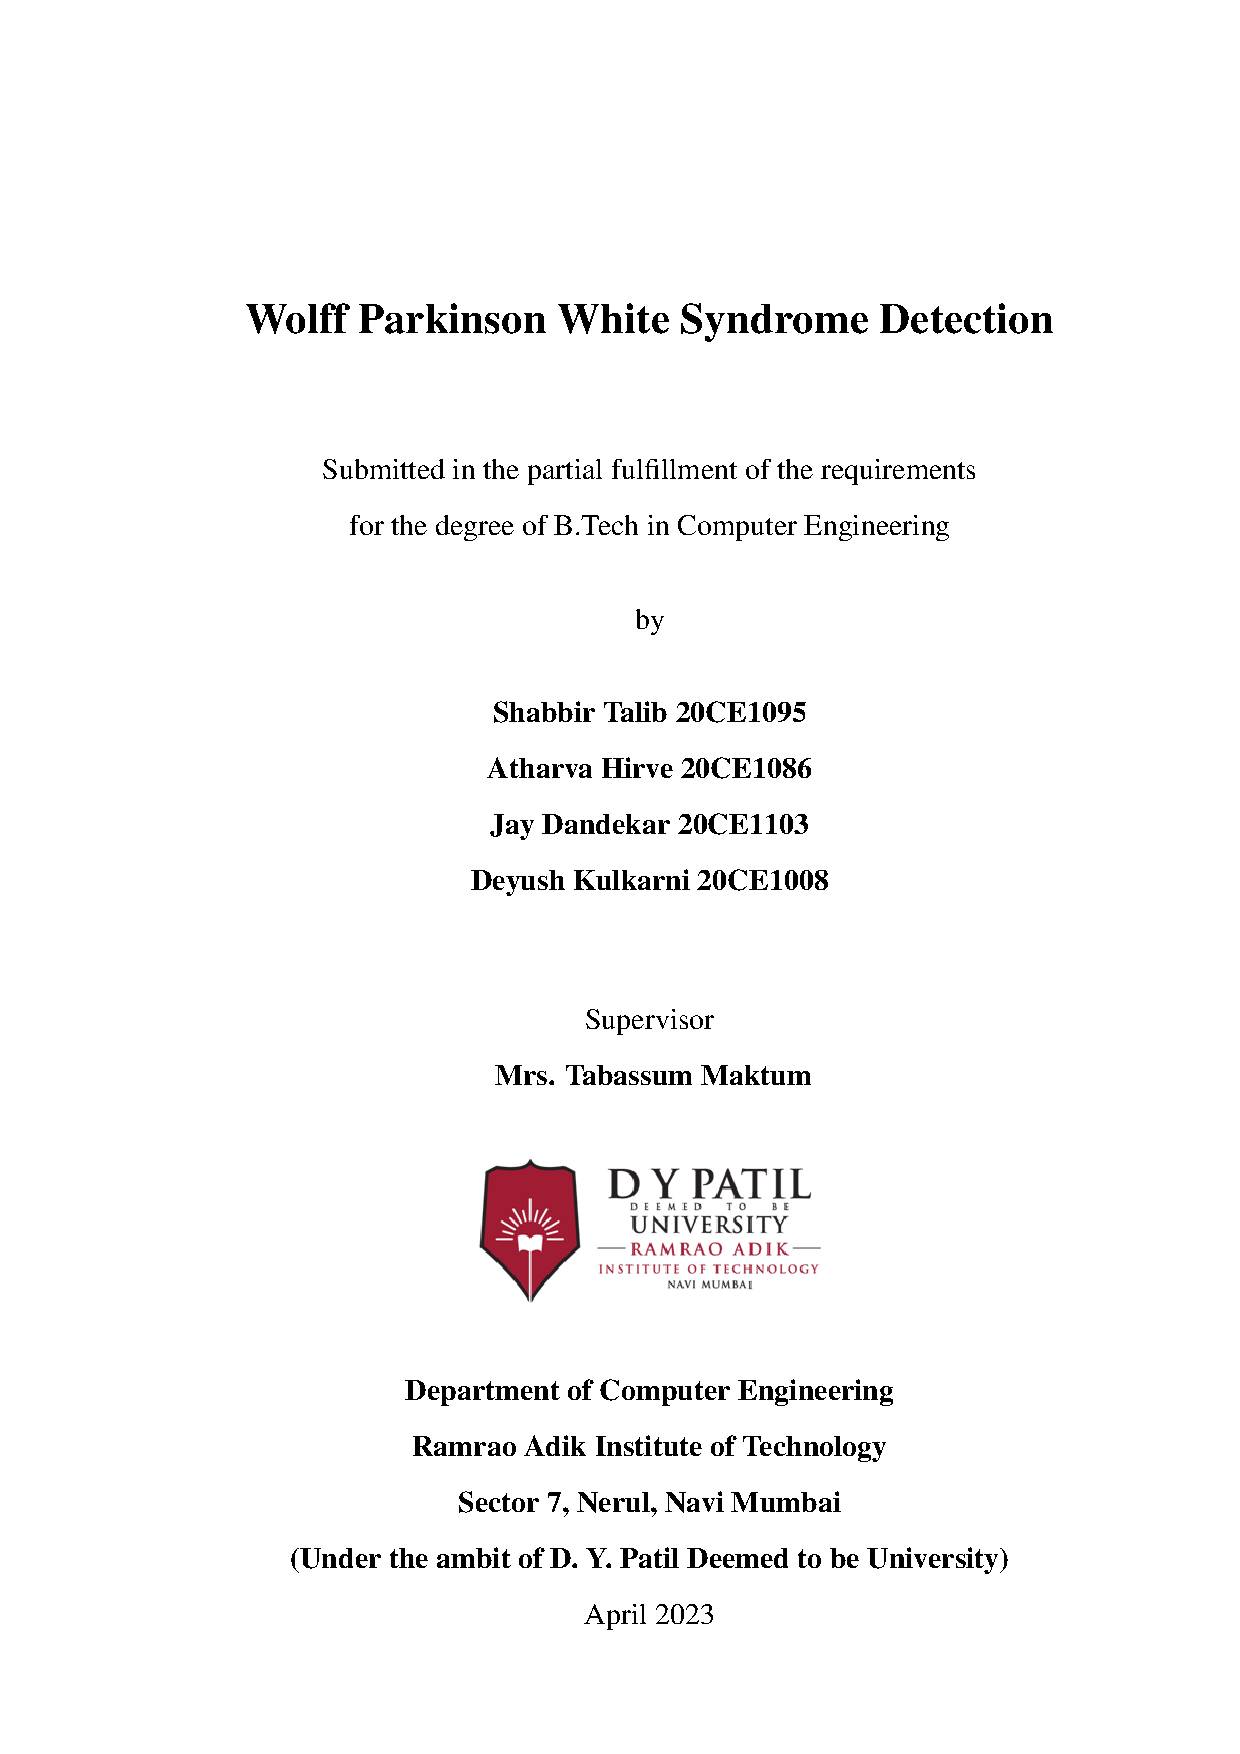
\includepdf[pages=-,pagecommand={},width=\textwidth]{report.pdf}
\newpage
\chapter{Publication Details / Copyright / Project Competitions}
\begin{enumerate}
	\item  S. Gaud, S. Kale, R. Sarambale, P. Gunjgur, “A Recommendation System for Integrated Agriculture Using Convolutional Neural Networks with Random Forest Algorithm,” Fifth International Conference on Computational Intelligence and Communication Technologies (CCICT), July 2022. [Published]
\end{enumerate}

%=====================================================================
% PUBLICATIONS
%  publications if any may be listed after the literature cited.
%% \include{mypubs}

%=====================================================================
% ACKNOWLEDGMENTS
%   This is the last item in the thesis. It should be signed by
%   author, with date.
\begin{acknowledgments}\thispagestyle{plain}
\addcontentsline{toc}{chapter}{Acknowledgement}
I thank the many people who have done lots of nice things for me.
\end{acknowledgments}


\end{document}
